\documentclass{journal}

\usepackage{here}
\usepackage{float}
\usepackage{adjustbox}
\usepackage{makecell}
\usepackage{graphicx}
\usepackage{cite}
\usepackage{amsmath}
\usepackage{amssymb}
\usepackage{pifont}
\usepackage{enumitem}
\usepackage{url}
\usepackage{multirow}
\usepackage{etoolbox}
\usepackage{titlesec}
\usepackage{caption}
\usepackage{changepage}
\usepackage{dsfont}
\usepackage[latin1]{inputenc}
\usepackage{tikz}
\usepackage{array}
\usetikzlibrary{shapes,arrows}
\captionsetup[table]{skip=5pt}
\newcommand{\cmark}{\ding{51}}

\DeclareMathOperator\erf{erf}

\interdisplaylinepenalty=2500
\hyphenation{op-tical net-works semi-conduc-tor}
\patchcmd{\thebibliography}{\section*{\refname}}{}{}{}
\setcounter{secnumdepth}{4}
\titleformat{\paragraph}
{\normalfont\normalsize\bfseries}{\theparagraph}{1em}{}
\titlespacing*{\paragraph}
{0pt}{3.25ex plus 1ex minus .2ex}{1.5ex plus .2ex}


\begin{document}

\title{Dust grain potential calculator \\ \it{User manual}}
\author{Dogan Akpinar and George E. B. Doran}
\markboth{D. Akpinar \& G. E. B. Doran}
{Shell \MakeLowercase{\textit{et al.}}:}

\maketitle

\section{Setup}

\begin{itemize}
    \item Install the modules specified in \textit{requirements.txt}
    \item Open \textit{Dust\_grain\_potential\_calculator.py} and edit the base path on line 8
\end{itemize}

\section{Variable table}

\begin{table}[H]
    \begin{adjustwidth}{-2.5cm}{}
        \label{tab:ValueTable}
        \begin{tabular}{|c|c|c|c|c|c|c|} 
        \hline
        Variable name & Unit & Requirements & \makecell{Normalised \\ variable name} & \makecell{Normalisation \\ factor} & Default value & Variable\\
        \hline
        Electron temperature ($T_e$) & $K$ & $T_e > 0$ & - & - & - & Yes \\
        \hline
        Ion temperature ($T_i$) & $K$ & $T_i \geq 0$ & $\Theta$ & $T_e$ & - & Yes \\
        \hline
        Relative ion charge ($z$) & - & \makecell{$0 < z \leq z_{max}$ \\ z $\in \mathds{Z}$} & - & - & - & No \\
        \hline
        Ion mass ($m_i$) & $kg$ & $m_i > 0$ & $\mu^2$ & $m_e$ & - & No \\
        \hline
        \makecell{Electron number density \\ at infinity ($n_0$)} & $m^{-3}$ & $n_0>0$ & - & - & - & No\\
        \hline
        Dust grain radius ($a$) & $m$ & $a \geq 0$ & $\alpha$ & $\lambda_D = \sqrt{\frac{\varepsilon_0 k_B T_e}{n_0 e^2}}$ & - & Yes\\
        \hline
        Flow speed (v) & $ms^{-1}$ & v $\geq 0$ & $\upsilon$ & $\upsilon_B = \sqrt{\frac{z k_B T_e}{m_i}}$ & 0 & Yes \\
        \hline
        \end{tabular}
    \end{adjustwidth}
\end{table}

\begin{itemize}
    \item The potential $\phi$ is normally negative and is normalised to $\Phi = -\frac{e\phi}{k_B T_e}$ which is a positive quantity.
\end{itemize}

\section{Using the code}

\medskip

% Define block styles
\tikzstyle{decision} = [diamond, draw, fill=yellow!20, 
    text width=5em, text badly centered, node distance=3cm, inner sep=0pt]
\tikzstyle{block} = [rectangle, draw, fill=blue!20, 
    text width=7em, text centered, rounded corners, minimum height=4em]
\tikzstyle{resultBlock} = [rectangle, draw, fill=red!20, 
    text width=7em, text centered, rounded corners, minimum height=4em]
\tikzstyle{requirement} = [ellipse, draw, fill=green!20, 
    text width=4em, text centered, rounded corners, minimum height=4em]
\tikzstyle{line} = [draw, -latex']
\tikzstyle{cloud} = [draw, ellipse,fill=red!20, node distance=3cm,
    minimum height=2em]
    
\begin{tikzpicture}[node distance = 2cm, auto]
    % Place nodes
    \node [block] (init) {Do you want to use dimensionless variables (y/n)};
    \node [decision, below left of = init, node distance = 4cm] (decideY) {y};
    \node [decision, right of = init, node distance = 4cm] (decideN) {n};
    \node [block, below of = decideN, node distance = 3cm] (speciesInput) {Enter the plasma ion species};
    \node [decision, below of = speciesInput, node distance = 2.5cm] (decideSpecies) {[element]};
    \node [block, below of = init, node distance = 5.5cm] (variableInput) {Enter variables according to requirements};
    \node [decision, below right of = variableInput, node distance = 4cm] (variables) {variable};
    \node [decision, below left of = variableInput, node distance = 4cm] (number) {[number]};
    \node [requirement, below of = variables, node distance = 3cm] (variableCentre) {Variable already chosen};
    \node [requirement, left of = variableCentre, node distance = 3cm] (variableLeft) {Can be varied};
    \node [requirement, right of = variableCentre, node distance = 3cm] (variableRight) {Can not be varied};
    \node [block, below right of = variableCentre, node distance = 4cm] (Retry) {Enter variables according to requirements};
    \node [block, below of = variableLeft, node distance = 2.8cm] (variableChosen) {Variable chosen};
    \node [block, below of = variableChosen, node distance = 3cm] (nextVariable) {Repeat for the other variables};
    \node [resultBlock, below of = nextVariable, node distance = 3cm] (result) {Result};
    %\node [block, below right of = variableCentre, node distance = 4cm] (NextVariable) {Enter next variable};
    % Draw edges
    \path [line] (init) -- (decideY);
    \path [line] (init) -- (decideN);
    \path [line] (decideY) -- (variableInput);
    \path [line] (decideN) -- (speciesInput);
    \path [line] (speciesInput) -- (decideSpecies);
    \path [line] (decideSpecies) -- (variableInput);
    \path [line] (variableInput) -- (variables);
    \path [line] (variableInput) -- (number);
    \path [line] (variables) -- (variableCentre);
    \path [line] (variables) -- (variableLeft);
    \path [line] (variables) -- (variableRight);
    \path [line] (variableCentre) -- (Retry);
    \path [line] (variableRight) -- (Retry);
    \path [line] (variableLeft) -- (variableChosen);
    \path [line] (variableChosen) -- (nextVariable);
    \path [line] (number) |- (nextVariable);
    \path [line] (nextVariable) -- (result);
\end{tikzpicture}

To run the code, see the flow diagram above where the yellow boxes show exactly what 
to input into the terminal except [number] which means type a number and [element] 
which means enter the name or chemical symbol of an element e.g hydrogen/H. 
It is possible to use the SI prefixes as shown in the following table. 

\smallskip

\begin{table}[H]
    \begin{adjustwidth}{4cm}{}
        \label{tab:ValueTable}
        \begin{tabular}{|c|c|} 
        \hline
        Prefixes & Value \\
        \hline
        Y  & $1 \times 10^{24}$ \\
        \hline
        Z & $1 \times 10^{21}$ \\
        \hline
        E & $1 \times 10^{18}$ \\
        \hline
        P & $1 \times 10^{15}$ \\
        \hline
        T & $1 \times 10^{12}$ \\
        \hline
        G & $1 \times 10^{9}$ \\
        \hline
        M & $1 \times 10^{6}$ \\
        \hline
        k & $1 \times 10^{3}$ \\
        \hline
        m & $1 \times 10^{-3}$ \\
        \hline
        u & $1 \times 10^{-6}$ \\
        \hline
        n & $1 \times 10^{-9}$ \\
        \hline
        p & $1 \times 10^{-12}$ \\
        \hline
        f & $1 \times 10^{-15}$ \\
        \hline
        a & $1 \times 10^{-18}$ \\
        \hline
        z & $1 \times 10^{-21}$ \\
        \hline
        y & $1 \times 10^{-24}$ \\
        \hline
        \end{tabular}
    \end{adjustwidth}
\end{table}

\smallskip

It is also possible to type $5 \ast 10 \wedge 6$ for example which will be interpreted as 
$5 \times 10^{6}$. Entering temperatures with "ev" after the number will allow the temperature to be 
inputted in electron volts, for example, $5$ev will be interpreted as $57970K$. 
Typing "variable" will prompt the user to enter a maximum and minimum value which will 
produce a graph rather than a number as the result. Once "variable" has been inputted once it 
will be impossible to set another parameter as the variable. 

\section{Adding a new variable}

\smallskip

To add a new variable, the procedure is as follows:

\medskip

Copy the dictionary for flow speed on line 255 and paste it underneath the existing one. 
Change the values to reflect the new variable and remove all that do not apply. 
The requirement classes found above the dictionaries can be used to make requirements, to find how to do this, 
the other dictionaries in the code should provide sufficient examples. 

\begin{figure}[H]
\centering
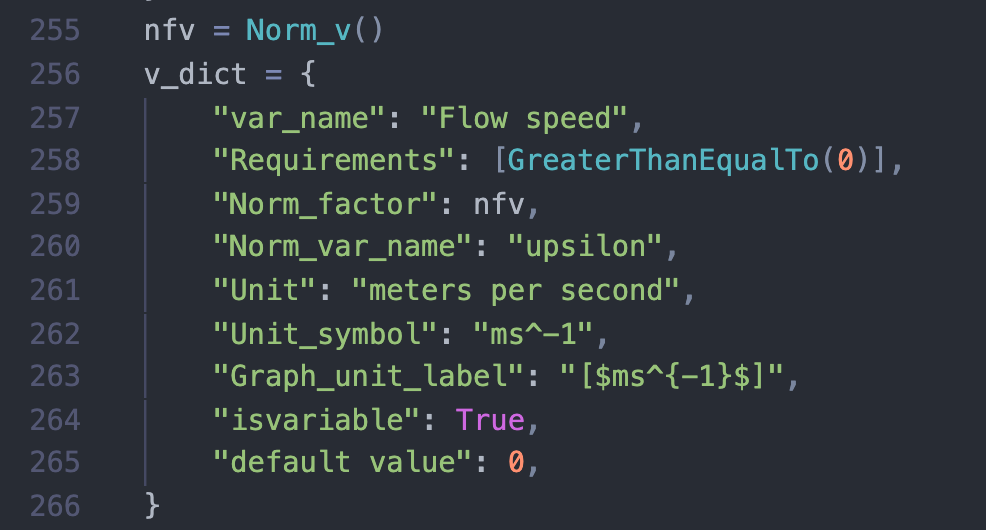
\includegraphics[width=\linewidth]{Output/code1.jpeg}
\label{code1} 
\end{figure}

All new variables should have a default value corresponding to the case where they are not considered, 
for example, not considering flow is to have a flow speed of zero. If a normalisation factor is required 
that depends on the other variables, then an object must be created above the new dictionary. This object 
will require a new class, to make this copy and paste the class for the flow velocity.

\begin{figure}[H]
\centering
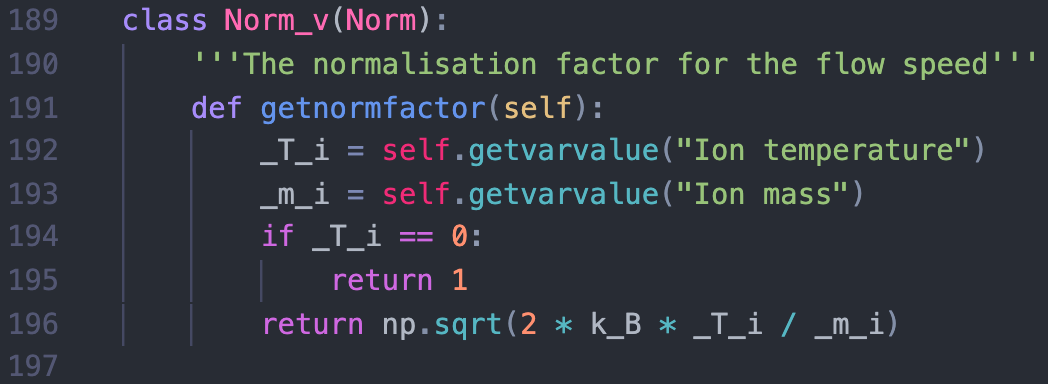
\includegraphics[width=\linewidth]{Output/code2.jpeg}
\label{code2} 
\end{figure}

Change the variables it collects for the ones required to make the 
normalisation factor. Note that if a value within the normalisation factor 
can be zero then it will cause a dividing by zero error, so something such as 
the code on lines 194-195 should be added to prevent this.

\newpage

Once the dictionary is complete add the name of the new dictionary to the list of dictionaries on line 269

\begin{figure}[H]
\centering

\includegraphics[width=\linewidth]{Output/code3.jpeg}
\label{code3} 
\end{figure}

\section{Adding a new model}

To add a new model, open the models folder and create a 
new model as a \textit{.py} file. The name of the file must be 
the same as the name of the model. The model requires at 
least five functions; get\_name(), colour(), get\_info(), 
potential\_finder() and priority(). For simplicity, 
copy and paste \textit{OML.py} into the new model and 
change the details. 

\begin{figure}[H]
\centering
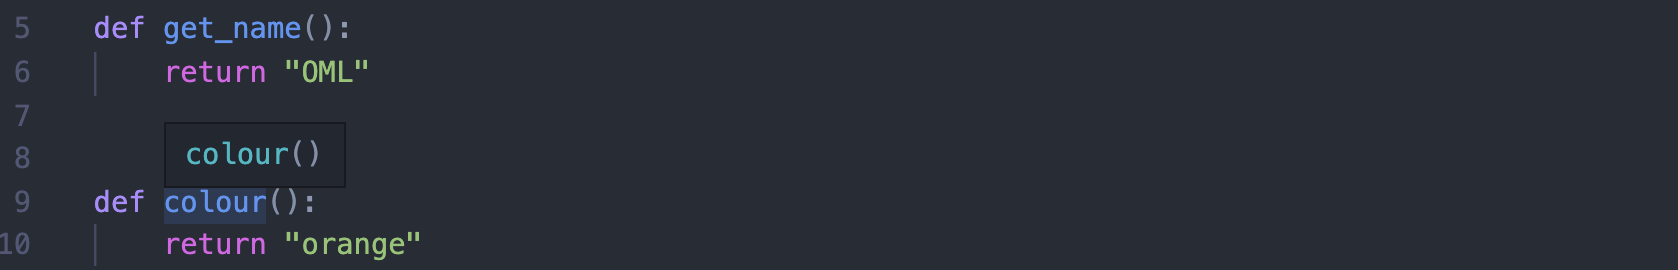
\includegraphics[width=\linewidth]{Output/code4.jpeg}
\label{code4} 
\end{figure}

Change the name in get\_name() to the new name and 
change the colour to whatever colour you want the 
model to be displayed as on a graph.

\begin{figure}[H]
\centering
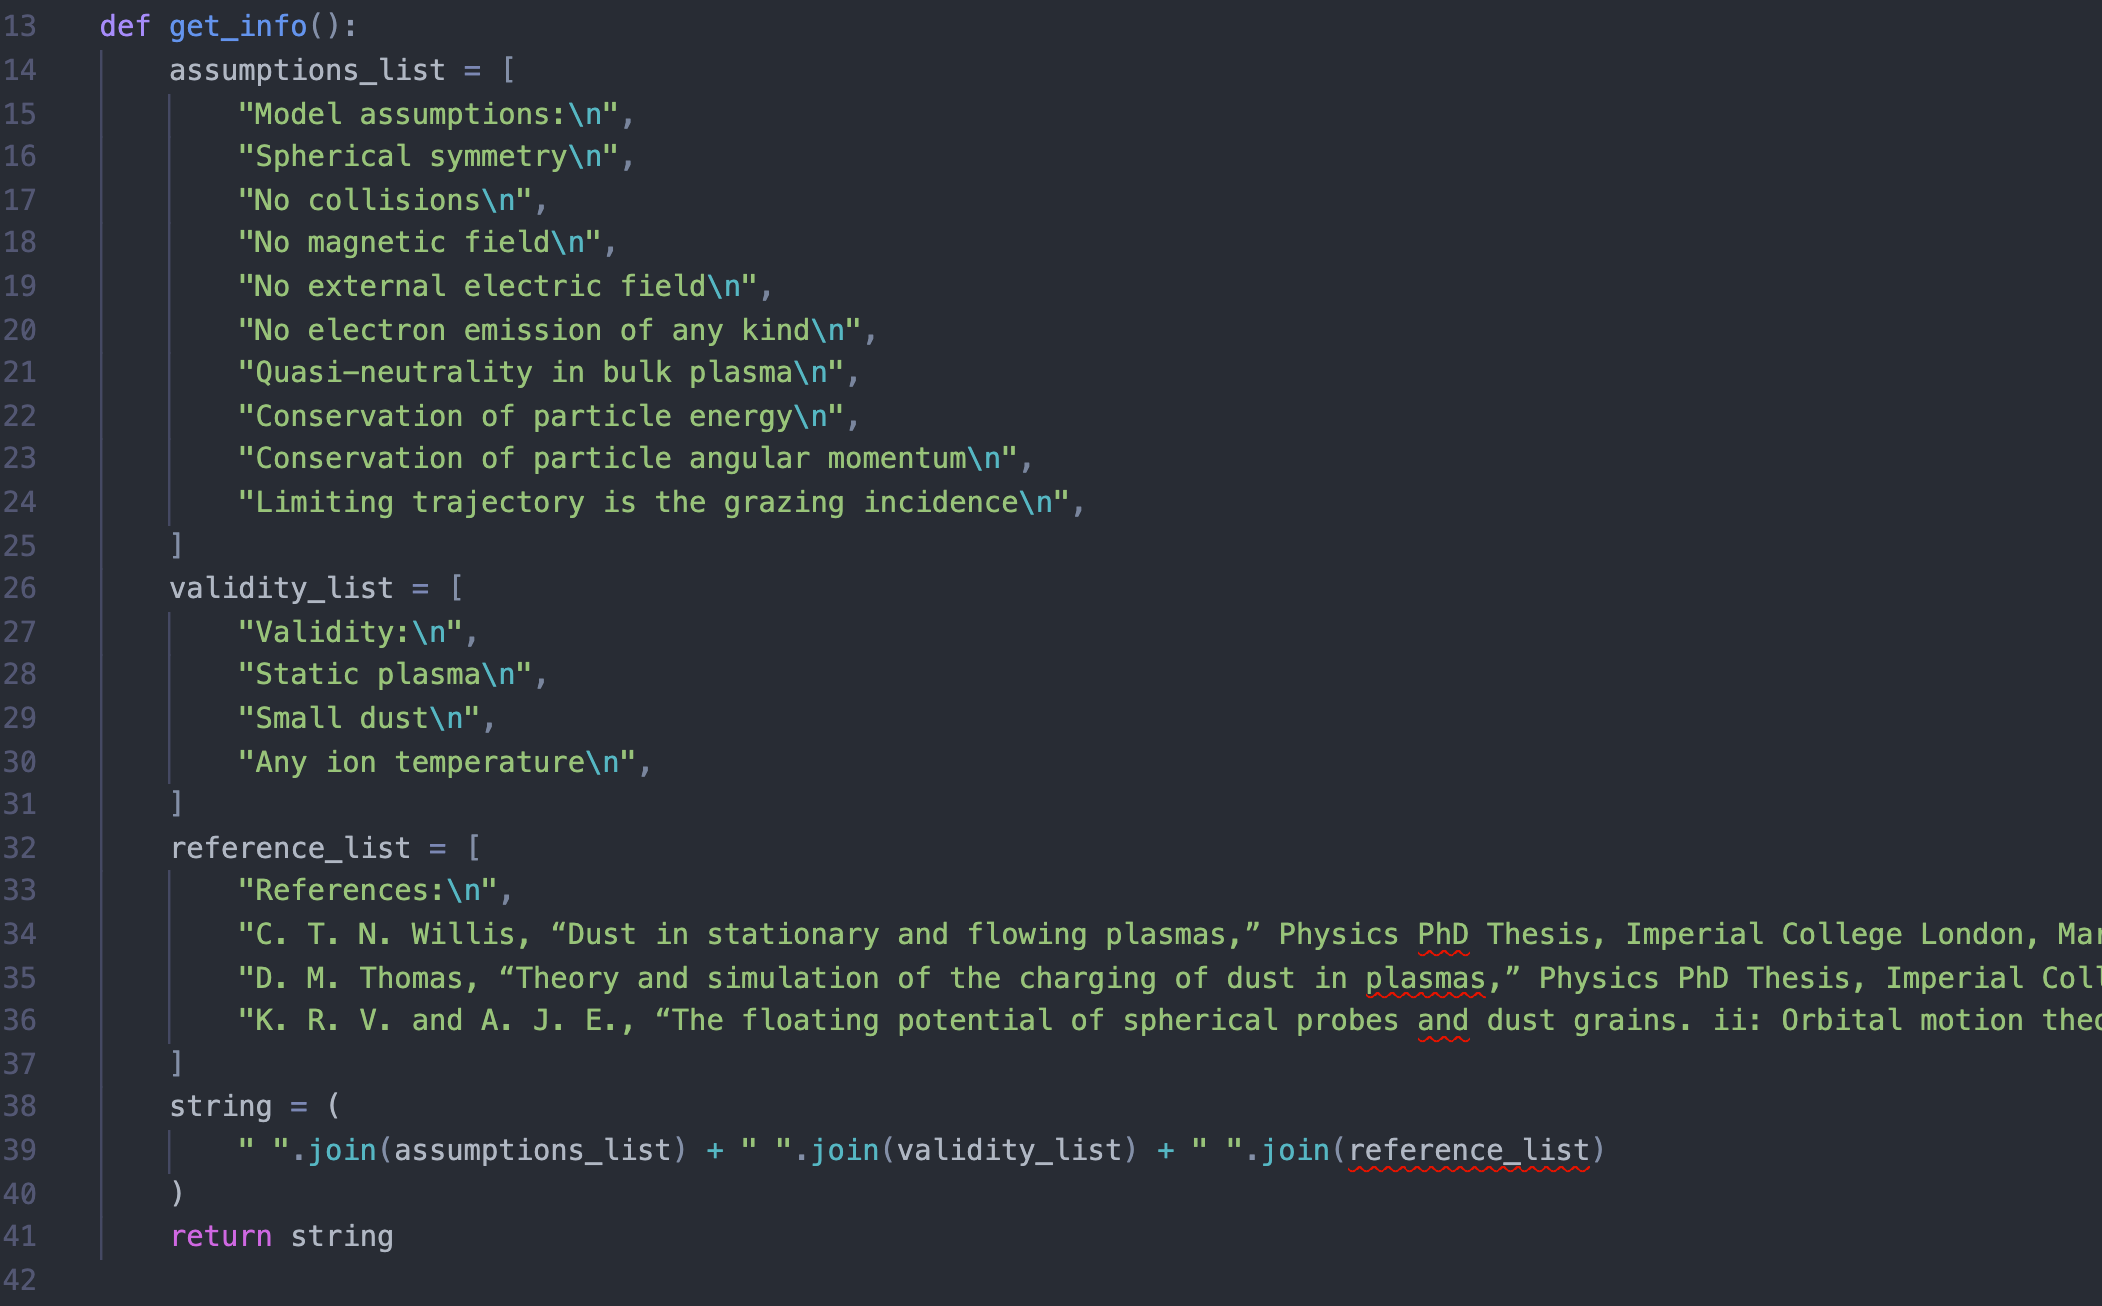
\includegraphics[width=\linewidth]{Output/code5.jpeg}
\label{code5} 
\end{figure}

The function get\_info() should include all the assumptions 
made by the model, the range of parameters it is valid 
over, a reference to where to find the model and any other 
information that the user may wish to know about the model.

\begin{figure}[H]
\centering
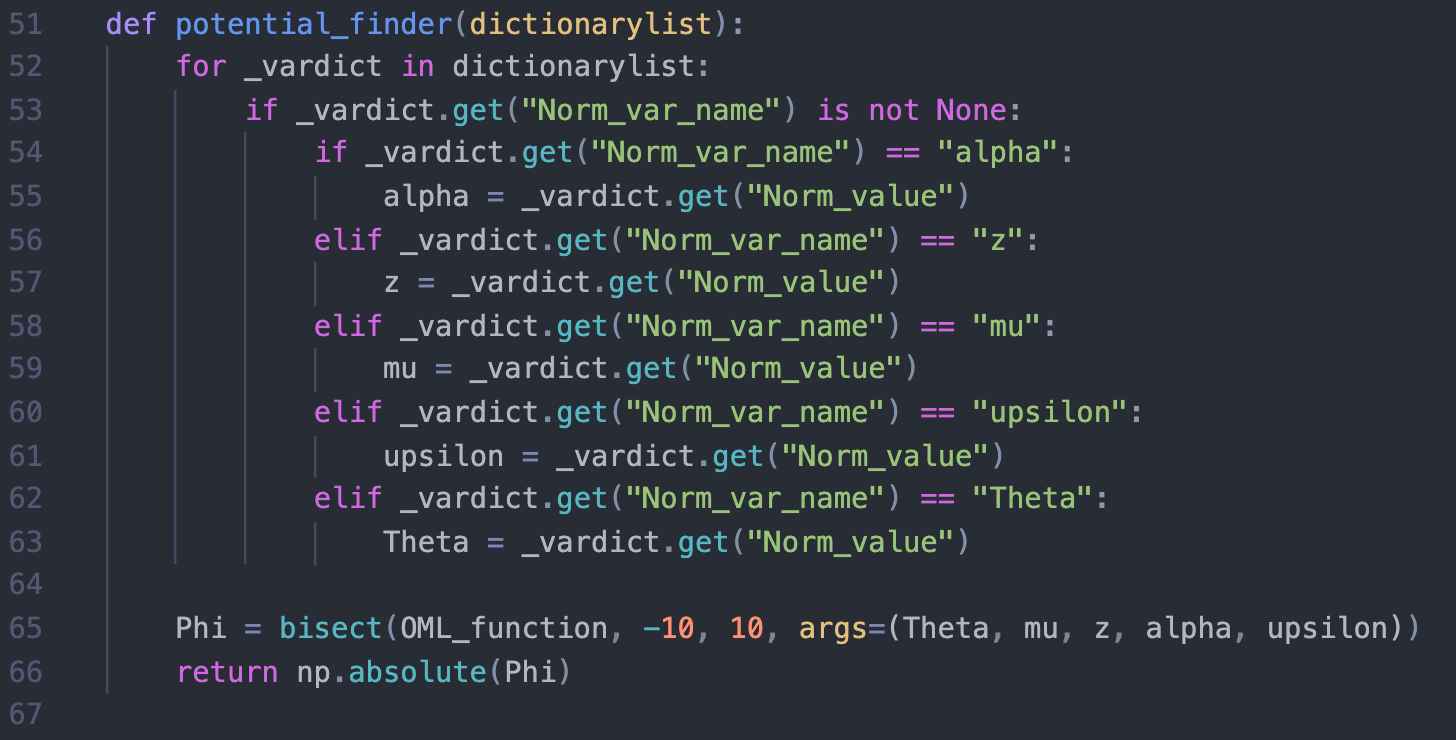
\includegraphics[width=\linewidth]{Output/code6.jpeg}
\label{code6} 
\end{figure}

The potential\_finder() function collects all the variables it needs 
to calculate the potential like so. All required variables should be 
collected in this way. Note the output should have the potential normalised 
in the same way as the existing models, $\Phi = -\frac{e\phi}{k_B T_e}$.

\begin{figure}[H]
\centering
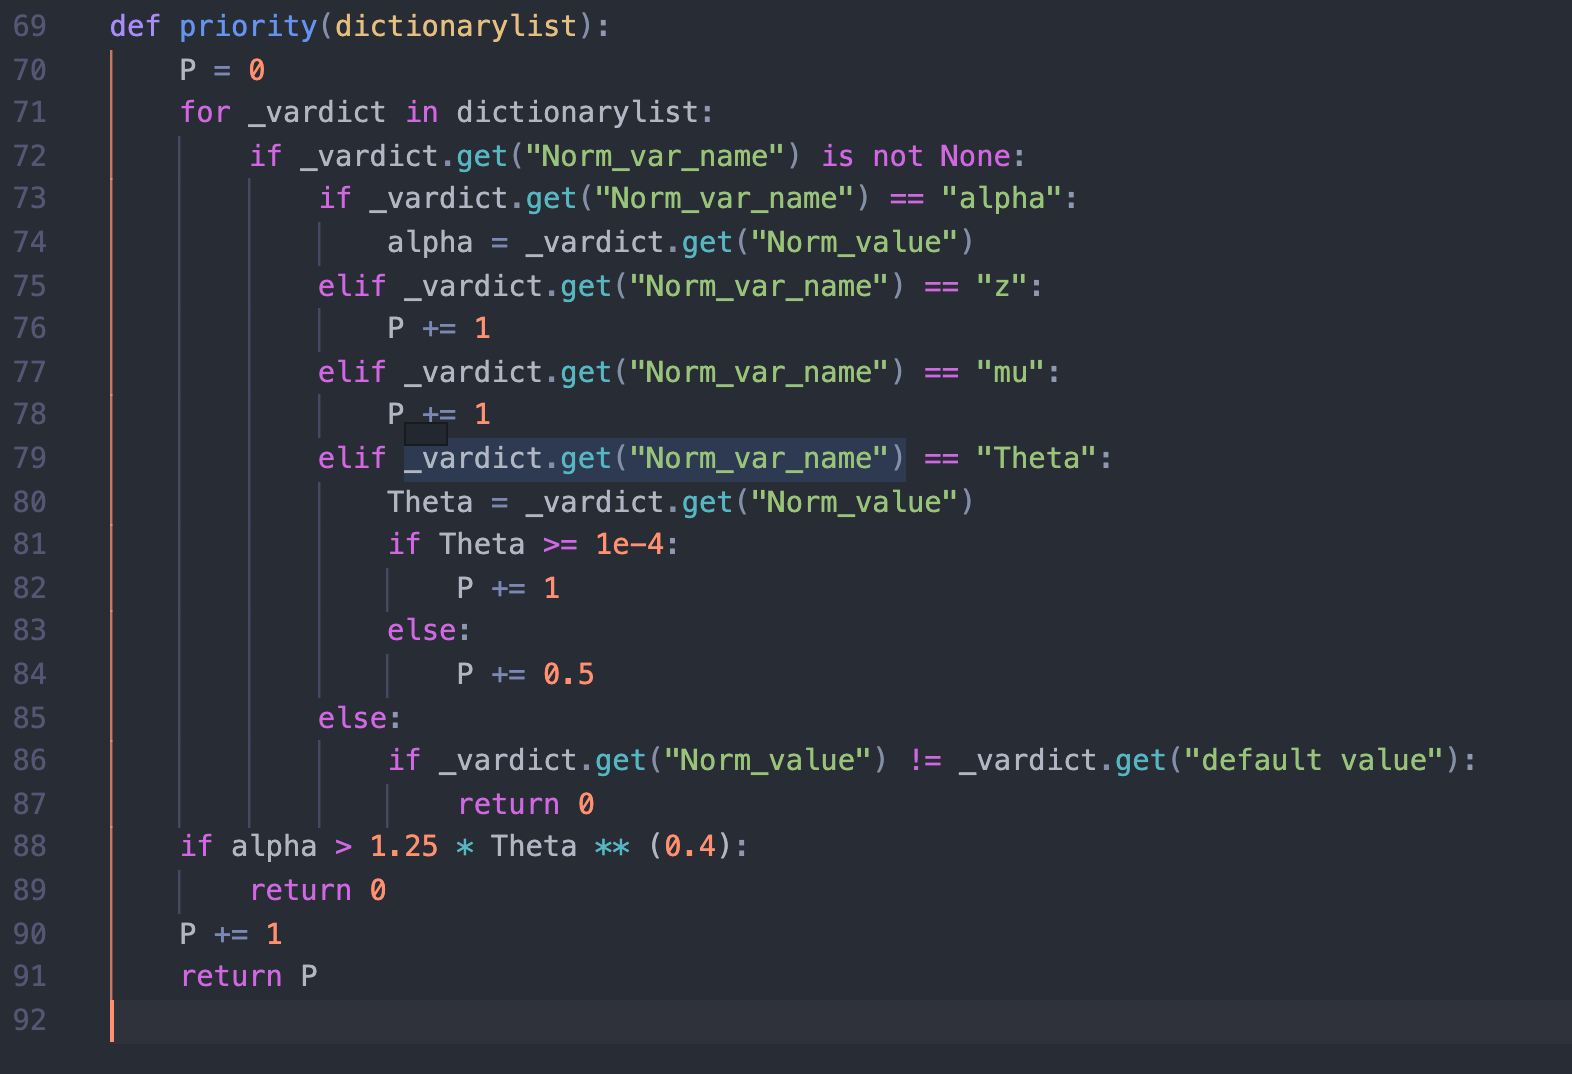
\includegraphics[width=\linewidth]{Output/code7.jpeg}
\label{code7} 
\end{figure}

The priority function deals with which model will be chosen for a 
given set of inputs. For the new priority function the variables should be 
collected as shown, if they are within the accepted range the priority value 
should increase by one and return a zero otherwise. Any input without a restriction 
should still be added and increase the priority function by one. To account for variables 
added after the creation of the model lines 85-87 should be included such that if there is 
an input variable not in the list of expected input variables that is not equal to its default 
value then the priority will be set to zero and the model will not be used. For example if the 
flow speed is not zero (its default value) then OML will have a priority of zero and will not be 
used. 

\end{document}